\documentclass[oneside]{article}

\usepackage{siunitx}
\usepackage{enumerate}
\usepackage{fancyhdr}
\usepackage{minted}
\usepackage{lastpage}
\usepackage{tcolorbox}
\usepackage{booktabs}
\usepackage{amsmath}
\usepackage[colorlinks=true]{hyperref}
\usepackage{caption} 
\captionsetup[table]{skip=5pt}
\usepackage{setspace}
\usepackage[absolute]{textpos}
\usepackage{xepersian} % Always last package to load

\settextfont{XW Zar}
\setlatintextfont{Adobe Garamond Pro}
\setlatinmonofont[Scale=0.8]{Monaco}
\defpersianfont\nastaliqfont{IranNastaliq}
\setlength{\TPHorizModule}{1cm}
\setlength{\TPVertModule}{1cm}
\linespread{1.5}
\pagestyle{fancy}
\renewcommand{\headrulewidth}{0pt}
\newcommand*{\fancypagenumber}{%
\fancyfoot[C]{صفحه
\thepage
از
\pageref{LastPage}}
}
\fancypagenumber
\fancypagestyle{plain}{\fancypagenumber}
% insert syntax highlighted code from a file
\newcommand{\inputcode}[2]{\inputminted[mathescape,%
                                                 linenos=false,%
                                                 formatcom=\small\setstretch{1}]{#1}{#2}}%
%\renewcommand{\theFancyVerbLine}{\sffamily\scriptsize
%\textcolor[rgb]{0.5,0.5,1.0}{\oldstylenums{\arabic{FancyVerbLine}}}}
\renewcommand{\textfraction}{0.05}
\renewcommand{\topfraction}{0.8} 
\renewcommand{\bottomfraction}{0.8} 
\renewcommand{\floatpagefraction}{0.8}
\title{تشخیص حروف به کمک پردازش تصویر}
\author{سارا قائمی , امین انصاریان }
\begin{document}
\maketitle\thispagestyle{empty}
\begin{textblock}{5}(6.5,2)\nastaliqfont
\noindent\Large
بسم الله الرحمن الرحیم
\end{textblock}

\section{فاز اول: تشخیص مشت و رسم اولیه به کمک 
\lr{OpenCV}}
در مرحله اول بر روی 
\lr{Anaconda}
راه اندازی 
\lr{OpenCV}

انجام شد. برای هرگونه تشخیص دست یا مشت در پردازش تصویر، چندین راه وجود دارد، يكی از راه حل های ابتدايی، توجه به رنگ پوست دست می باشد. رنگ پوست خصیصه بسیار خوبی برای تشخیص دست میباشد. اگر در تصویر ورودی از دوربین کامپیوتر با استفاده از فیلتر های خاص، قسمت هایی که رنگ دست دارد را به رنگ سفید، و بقیه قسمت ها را به رنگ مشکی نشان دهیم، میتوان به راحتی دست را در تصویر تشخیص داد. اما این روش مشکل های متعددی دارد. مهم ترین مشکل این روش، همرنگ بودن صورت انسان با دست او میباشد. اگر در تصویر دوربین، صورت شخص هم حاضر باشد، پس از گذشتن از فیلتر، صورت هم به رنگ سفید نمایش داده خواهد شد. مشکل دوم این روش این است که باید لباس آستین دار به تن داشت. البته در این روش با استفاده از بعضی فیلتر ها، با توجه به بزرگتر بودن سر از دست، قادر به تشخیص دست از سر شده اند. ولی اگر دست به تصویر نزدیکتر باشد این روش هم با مشکل مواجه میشود. خروجی فیلتر تشخیص رنگ بدن که توسط افراد مختلف پیاده سازی شده است را در  شکل
\ref{figHand1}
و
\ref{figHand2} 
میبینید.

روش استفاده شده در این پروژه، استفاده از تعداد زیادی از لایه های پست سر هم قرار گرفته از 
\lr{classifier}
های ضعیف دست میباشد.
\begin{figure}
\centering
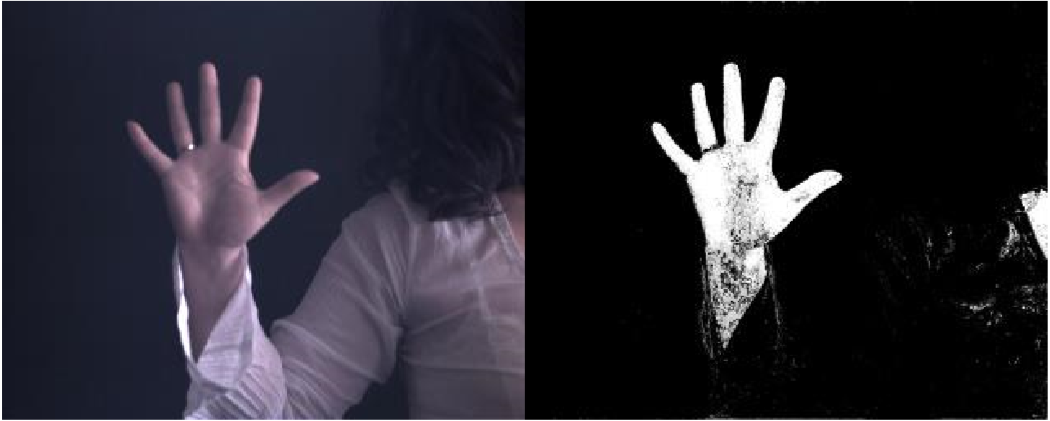
\includegraphics[width=0.6\textwidth]{Pictures/1.png}
\caption{تشخیص رنگ بدن}
\label{figHand1}
\end{figure}

\begin{figure}
\centering
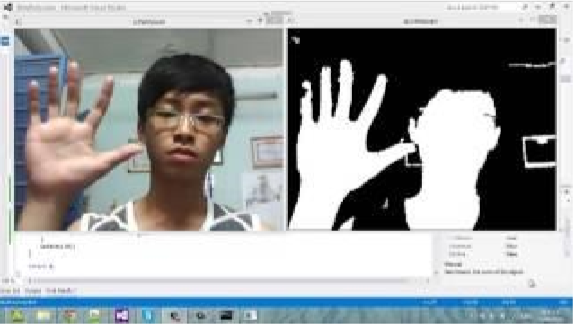
\includegraphics[width=0.6\textwidth]{Pictures/2.png}
\caption{تشخیص رنگ بدن}
\label{figHand2}
\end{figure}

\subsection{فایل های 
\lr{xml}}
برای تشخیص مشت در یک تصویر دوربین میبایست تعداد زیادی نمونه عکس که شامل نمونه های درست و غلط میباشد توسط الگوریتم های 
\lr{machine learning}
آموزش داده شود(
\lr{train}
شود).
منظور از نمونه های درست عکس هایی هستند که مشت در آن ها وجود دارد و منظور از نمونه های غلط عکس هایی هستند که مشت در آن ها وجود ندارد.

برای 
\lr{train}
تشخیص دهنده(فایل
\lr{xml}
) مجموعه ای شامل حدود 500 عکس مشت از اعضای آزمایشگاه تهیه شد و در تمامی این عکس ها، ناحیه دست به دقت مشخص گردید.  سپس مجموعه شامل حدود 500 عکس از محیط آزمایشگاه و اطراف آزمایشگاه و صورت ها و لباس ها و رنگ های مختلف بدون حضور هیچ دستی تهیه شد.

در این پروژه از این فایل برای تشخیص مشت استفاده شد. 
\subsection{تشخیص مشت}
بر روی فایل 
\lr{xml}
اشاره شده در زیربخش قبلی، یک 
\lr{CascadeClassifier}
اجرا میشود. 
\lr{CascadeClassifier}
از تعدادی مرحله تشکیل شده است که هر مرحله شامل گروهی از تشخیص دهنده های ضعیف است. این تشخیص دهنده های ضعیف، طبقه بندی های ساده ای هستند که میتوانند با درصد صحت پایین، وجود و یا عدم وجود شی مورد نظر در عکس را مشخص میکند. هر مرحله از 
\lr{CascadeClassifier}
توسط تکنیکی موسوم به
\lr{ Boosting }
آموزش داده میشوند.
\lr{ Boosting}
 قابلیت آموزش یک تشخیص دهنده قوی از تعدادی تشخیص دهنده های ضعیف را حاصل میکند.
\lr{ Boosting}
با استفاده از میانگین گیری وزن دار از تشخیص های ضعیف گرفته شده، یک تشخیص قوی تر درباره حضور و یا عدم حضور شی مورد نظر در تصویر میدهد. 

باید توجه داشت که برای پیاده سازی اکثر الگوریتم های پردازش تصویر ابتدا تصویر را سیاه و سفید میکنند که به این منظور 
\lr{OpenCV}
خود تابعی را در اختیار قرار داده است. 

پس از تغییر رنگ تصویر، تابع 
\lr{detectMultiScale}
بر روی هر 
\lr{frame}
تصویر اجرا میشود. شیوه کار این تابع به این صورت است که تصویر را به نواحی مستطیلی که با هم همپوشانی دارند تقسیم کرده و با این کار تصویر را جارو میکند. که نتیجه آن مختصات مستطیل خروجی ای است که بالاترین شباهت را به مشت دارد. این تابع پارامتر هایی قابل تنظیم برای عملکرد خود در اختیار برنامه نویس قرار میدهد. از مهم ترین این پارامتر ها میتوان به 
\lr{scaleFactor}
که مقیاس کاهش اندازه در تصویر میباشد،
\lr{minNeighbors}
که حداقل تعداد همسایه برای هر مستطیل را مشخص میکند،
\lr{minSize}
که حداقل اندازه مستطیل برای اینکه مشت باشد را میدهد اشاره کرد.

در انتهای برای نشان دادن مشت های تشخیص داده شده با استفاده از خروجی تابع فوق مستطیلی به دور مشت رسم میشود. 
در فاز اول فقط این مختصات ها ذخیره شده و سپس در یک نمودار جداگانه با استفاده از کتابخانه
\lr{matplotlib}
 رسم میشود.

دو نمونه از خروجی کد فاز اول در شکل
\ref{Phase11}
و
\ref{Phase12}
آمده است

\begin{figure}
\centering
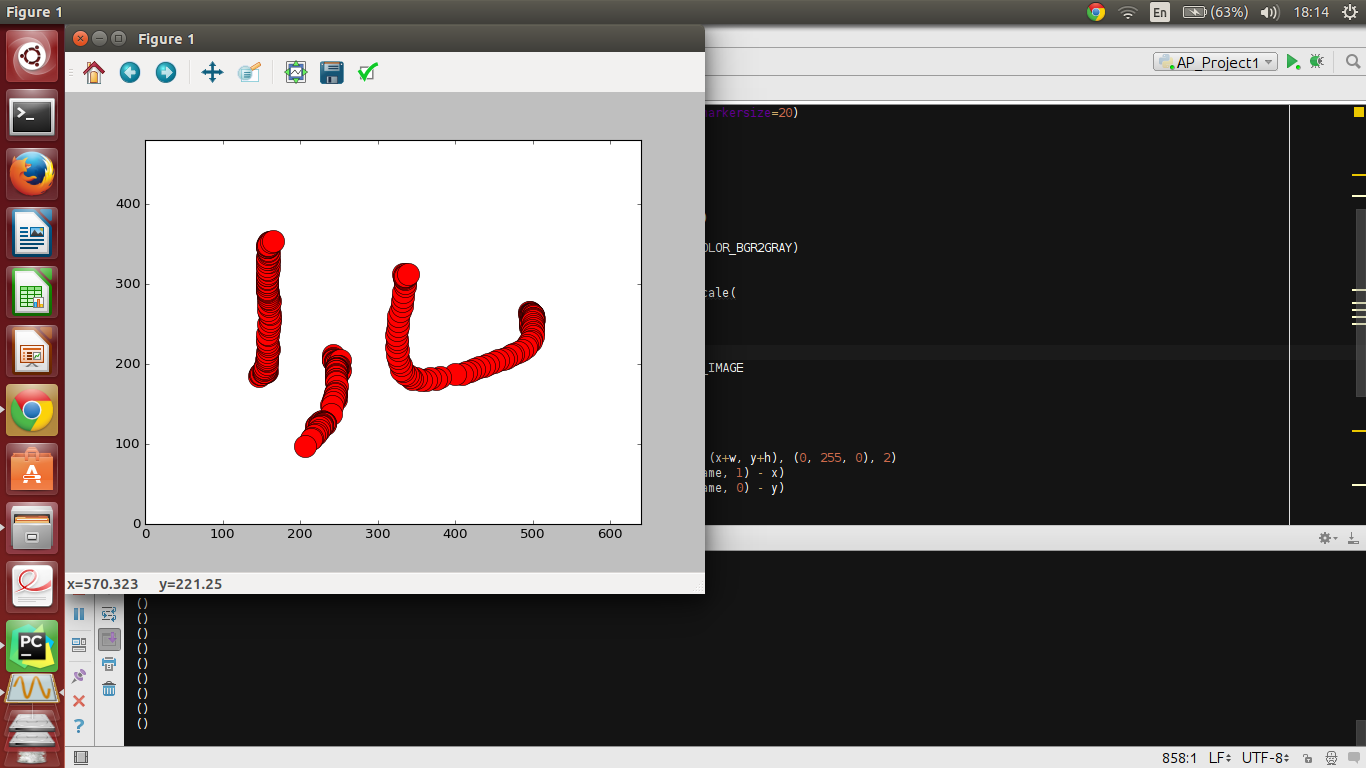
\includegraphics[width=0.6\textwidth]{Pictures/3.png}
\caption{نمونه اجرای فاز 1}
\label{Phase11}
\end{figure}

\begin{figure}
\centering
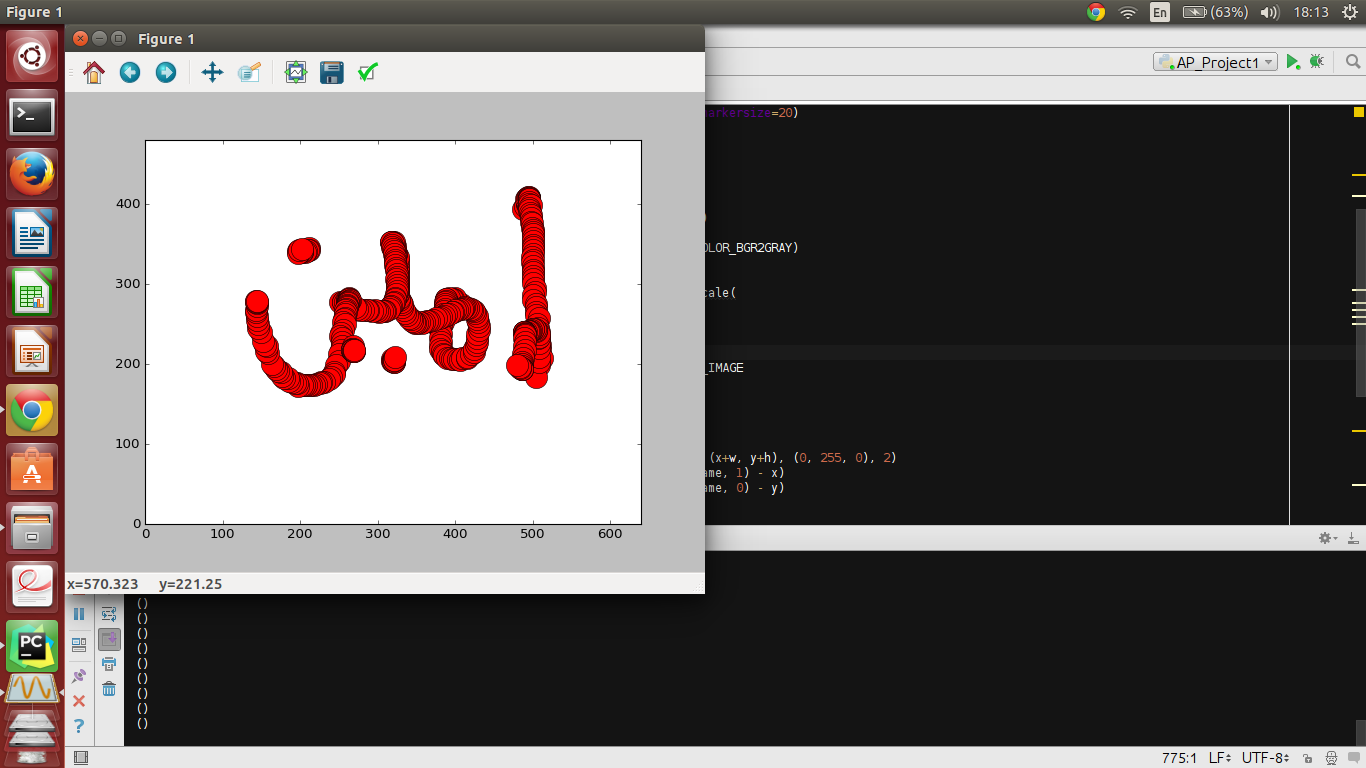
\includegraphics[width=0.6\textwidth]{Pictures/4.png}
\caption{نمونه اجرای فاز 1}
\label{Phase12}
\end{figure}

\section{فاز 2: رسم بلادرنگ نمودار و 
\lr{GUI}}
در این فاز بخش پردازش تصویر تغییری نکرده و فقط به رسم بلادرنگ(
\lr{realtime}
) نمودار پرداخته شده است. همچنین در محیط 
\lr{Qt Designer}
یک 
\lr{GUI (Graphical User Interface)}
یا رابط کاربری گرافیکی طراحی شد.

\subsection{\lr{GUI}}
برای طراحی 
\lr{GUI}
برای نشان دادن تصویر هر 
\lr{frame}
از یک 
\lr{label}
استفاده شده است. همچنین برای بخش نمودار هم از
\lr{label}
استفاده شده است. نحوه استفاده از هرکدام در بخش کد نمودار بلادرنگ آمده است. نمونه ای از عکس این رابط کاربری در شکل
\ref{GUI}
آمده است.
\begin{figure}
\centering
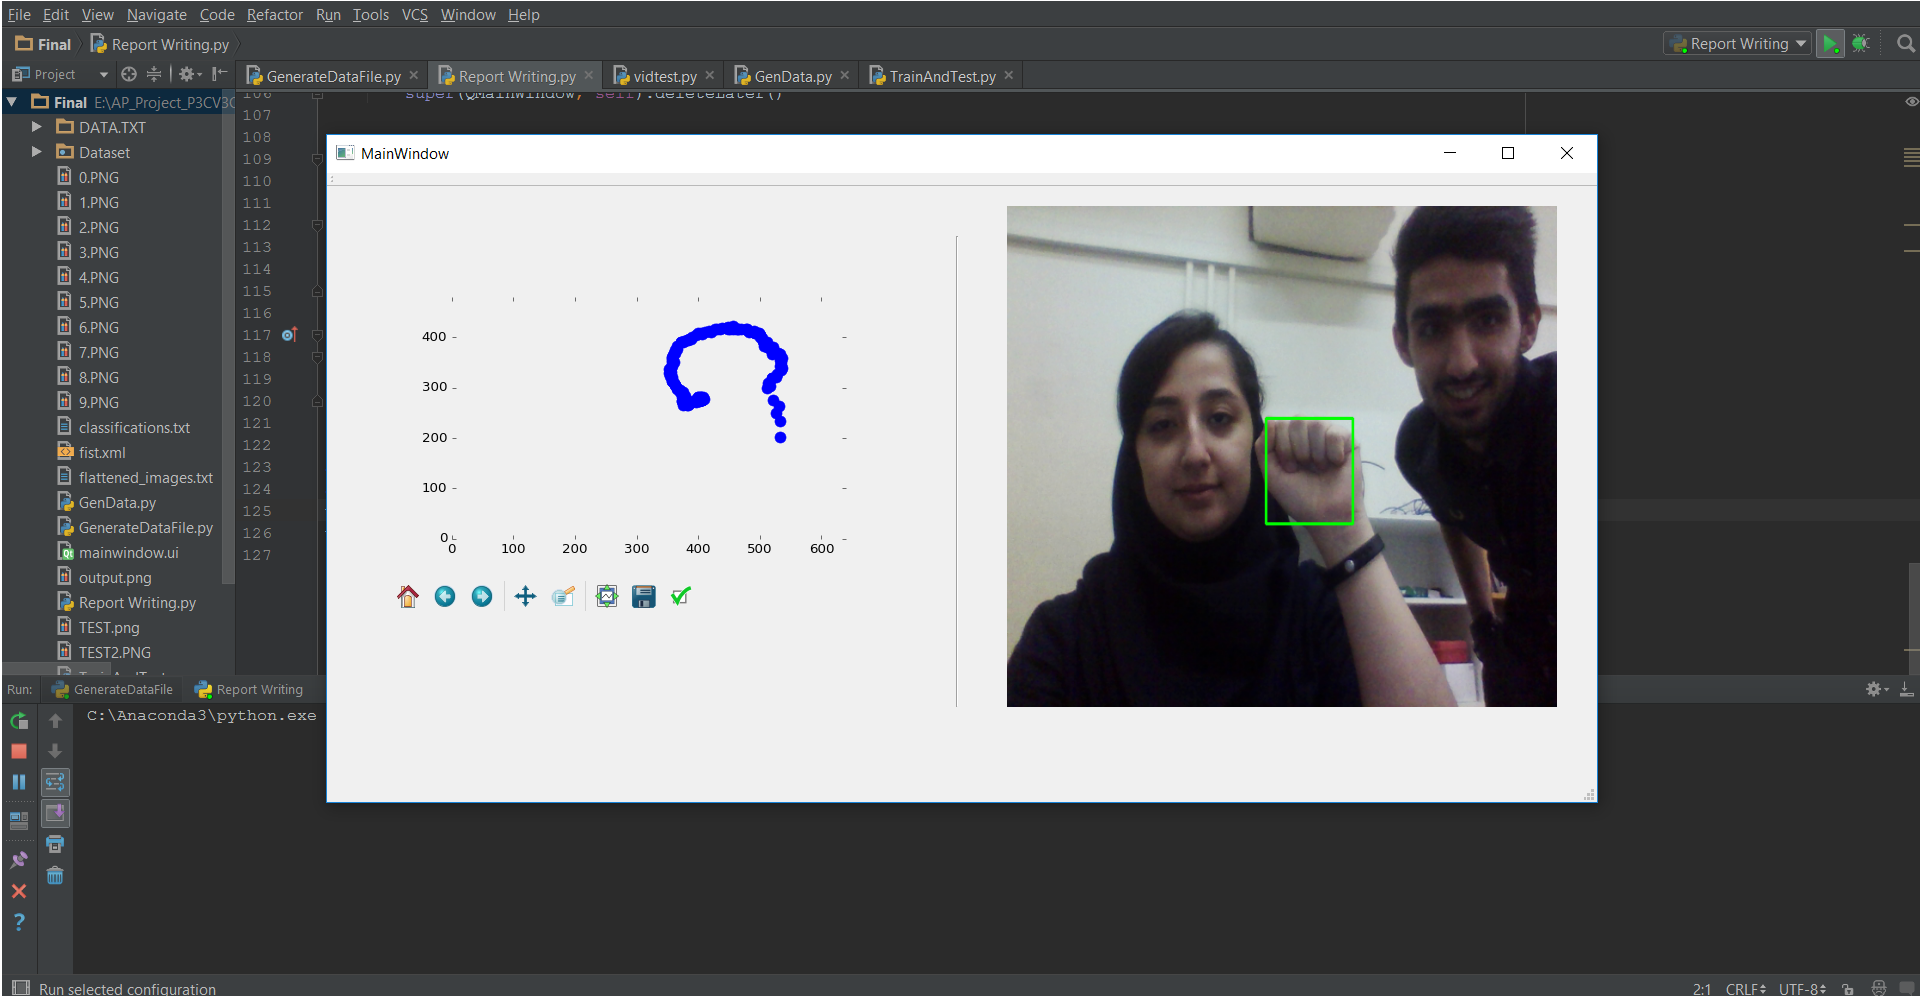
\includegraphics[width=0.6\textwidth]{Pictures/5.png}
\caption{GUI}
\label{GUI}
\end{figure}

\subsection{Realtime Plot}
برای اینکه بتوان به صورت بلادرنگ نمودار نقاط مشت ها را رسم نمود باید بخش نمودار را در یک 
\lr{Thread}
جداگانه انجام داد.

کد فاز دوم در کل شامل 3 کلاس اصلی میباشد. یکی کلاس 
\lr{ControlWindow}
که در واقع کلاس مربوط به 
\lr{GUI}
است و کلاس اصلی محسوب میشود، کلاس دوم کلاس
\lr{QtCapture}
که در آن پردازش های مربوط به پردازش تصویر صورت میگیرد، و آخری کلاس
\lr{PlotThread}
که کار رسم نمودار بلادرنگ را انجام میدهد.
در این پروژه برای رسم بلادرنگ نمودار همان طور که در کلاس به تفضیل توضیح داده شده بود عمل شده است. نکته قابل توجه در این بخش از کد آن است که برای دسترسی به مختصات های مشت ها چون در 
\lr{QtCapture}
هستند در 
\lr{ControlWindow}
برای رسم نمودار دسترسی وجود نداشت. به این منظور از مفهوم 
\lr{Pass by Reference}
استفاده شده است و با توجه به اینکه 
\lr{list}
در پایتون 
\lr{mutable}
هستند بنابراین 
\lr{Pass by Reference}
میشوند.
\section{فاز سوم: تهیه بانک داده ، آموزش آن و تشخیص حروف و اعداد}
پس از رسم بلادرنگ نمودار در فاز قبل حال به سراغ بخش تشخیص متن از روی دست خط می رویم، شیوه ی کلی کار به این صورت است که در ابتدا با استفاده از الگوریتم های یادگیری ماشین(
\lr{Machine Learning}
) یک بانک داده از نمونه هایی که توسط دست کشیده شده اند، تهیه می شود. سپس با استفاده از آموزش این بانک (
 \lr{dataset}
) متن از روی نوشته تشخیص داده می شود که به تفصیل بیان خواهد شد.
\subsection{طراحی دیتاست،تهیه دیتاست}
ابتدا مجموعه بزرگی از نمونه های مختلف برای حروف و اعداد تهیه شد. در شیوه ی معمول به این صورت می باشد که به اندازه 10 برابر تعداد پیکسل های هر نمونه ی مورد بررسی (در اینجا 10*28*28) نمونه برای دقت بالای کار نیاز می باشد که به علت حجم بالای آن و  ضیق وقت، تنها به تعدادی از حروف (
\lr{A,B,E,H,I,M,N,O,P,R,S,Z}
) و اعداد، در تعداد نمونه در حدود 60 عدد اکتفا شد که نمونه ی آن برای حرف
\lr{A} 
در شکل 
\ref{A}
آمده است.
\begin{figure}
\centering
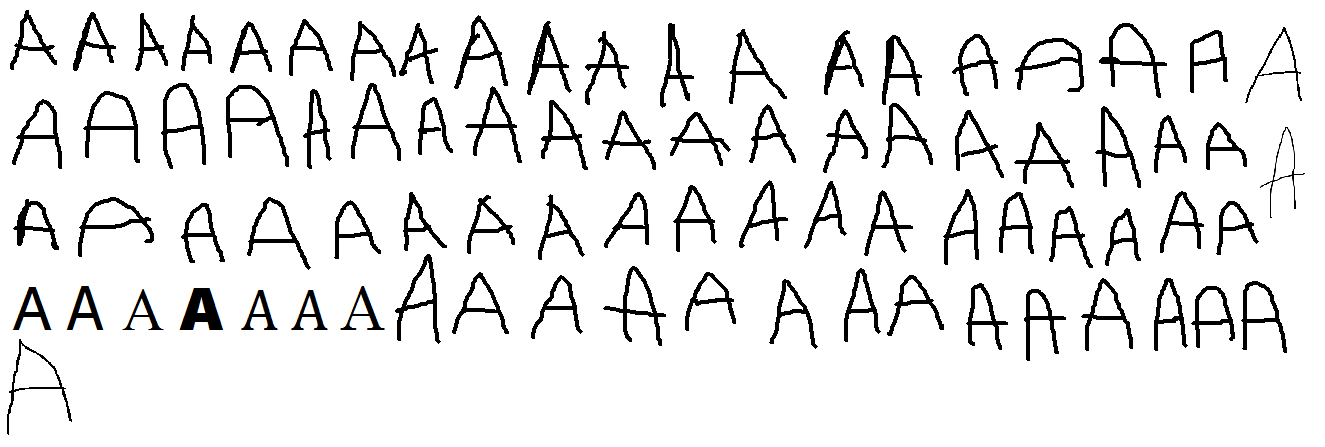
\includegraphics[width=0.6\textwidth]{Pictures/6.png}
\caption{نمونه حرف
\lr{A}}
\label{A}
\end{figure}

حال به بررسی شیوه تهیه دیتاست می پردازیم

پس از اعمال فیلتر سیاه و سفید بر روی عکس آن را از یک فیلتر عبور می دهیم به صورتی که تنها رنگ سفید از آن خارج شود، سپس با مشتق گرفتن از عکس، لبه های آن خارج شده و درواقع به دور هرکدام از آیتم های بالا یک کانتور(حلقه بسته) کشیده می شود، از این کانتور ها برای
 \lr{train} 
کردن استفاده می کنیم.

دیتاست مورد نظر از دو بخش ماتریس های حروف(
\lr{flattened images}
) و بخش بندی های مختلف(
\lr{classification}
) تشکیل شده است.

حال با استفاده از یک حلقه ، برای هر کانتور از کاربر حرف مورد نظر گرفته شده و سپس به آن نسبت داده می شود. باید در نظر داشت که هرکدام از عکس های کانتور ها را برای افزایش دقت، تغییر اندازه داده و کوچک می کنیم.

سپس هر کدام از کلید ها را را در فایل(
\lr{classification}
) به عنوان عدد اسکی آن ذخیره می نماییم و ماتریس عکس های تنظیم شده مورد نظر را نیز در (
\lr{flattened images}
) ذخیره می نماییم که در نهایت این دو در دو فایل متنی ذخیره می شوند و دیتاست ما آماده ی 

شدن می باشد. یک مرحله از تهیه دیتا ست به صورت شکل 
\ref{dataset}
 می باشد.
\begin{figure}
\centering
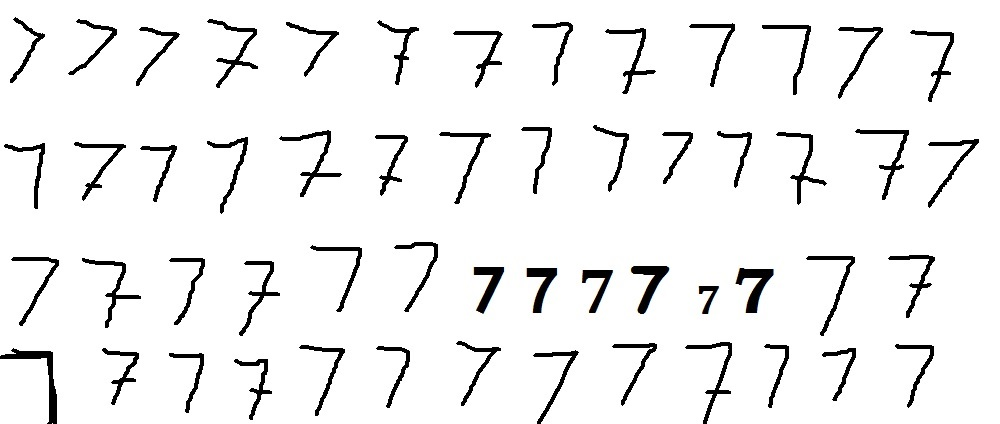
\includegraphics[width=0.6\textwidth]{Pictures/7.jpg}
\caption{تهیه دیتاست}
\label{dataset}
\end{figure}

\subsection{Training}
در این مرحله از الگوریتم ریاضی نزدیک ترین همسایه برای
\lr{train}
کردن استفاده می کنیم که در ابتدا به اختصار به توضیح آن می پردازیم

نزدیک‌ترین همسایه 
\lr{K Nearest Neighbor (KNN)}
:

روش
\lr{k}
نزدیک‌ترین همسایه یک گروه شامل 
\lr{k}
رکورد از مجموعه رکورد‌های آموزشی که نزدیک‌ترین رکورد‌ها به رکورد آزمایشی باشند را انتخاب کرده و بر اساس برتری رده یا برچسب مربوط به آن‌ها در مورد دسته رکورد آزمایشی مزبور تصمیم‌گیری می‌نماید. به عبارت ساده‌تر این روش رده‌ای را انتخاب می‎‌کند که در همسایگی انتخاب شده بیشترین تعداد رکورد منتسب به آن دسته باشند. بنابراین رده‌ای که از همه رده‌ها بیشتر در بین 
\lr{k}
نزدیک‌ترین همسایه مشاهده شود، به عنوان رده رکورد جدید در نظر گرفته می‌شود. ایده اصلی روش 
\lr{KNN}
این است که اگر موجودی مثل اردک راه برود و مثل اردک
\lr{quack quack}
کند، پس حتما یک اردک است. 

استفاده از الگوریتم 
\lr{KNN}
نیازمند تعیین سه موضوع می‌باشد: 

باید یک مجموعه رکورد داشته باشیم. 

- یک معیار محاسبه شباهت نیز باید داشته باشیم. 

- مقدار 
\lr{k}
نیز باید مشخص شود تا بتوان بر اساس آن عمل نمود. برای مسائل دسته بندی دودویی معمولا در نظر گرفتن مقادیر فرد برای 
\lr{k}
بهتر است. زیرا امکان پیروز شدن یکی از دو دسته را افزایش می‌دهد. برای مسائل رده‌بندی چند رده‌ای باید عدد
\lr{k}
را بزرگ‌تر از تعداد رده ها و نیز متفاوت با عدد تعداد رده‌ها از نظر زوج یا فرد بودن در نظر گرفت. یعنی اگر تعداد رده‌ها زوج باشدباید 
\lr{k}
نهایی را فرد در نظر گرفت و بالعکس. 

در رده‌بندی‌های 
\lr{KNN}
برای دسته‌بندی کردن یک رکورد با دسته نا‌مشخص به صورت زیر عمل می‌شود: 

- فاصله رکورد جدید از همه رکورد‌های آموزشی محاسبه می‌شود. 

- نزدیک‌ترین همسایه‌ها مشخص می‌شوند. 

- از برچسب دسته 
\lr{k}
نزدیک‌ترین همسایه، برای پیش‌بینی دسته رکورد جدید استفاده می‌شود. به این صورت که بین 
\lr{k}
رکورد رأی‌گیری شده و دسته‌ای که بیش‌ترین تعداد دفعات دیده‌شدن را در بین این
\lr{k}
رکورد داراست، به عنوان دسته رکورد جدید در نظر گرفته خواهد شد. انتخاب مقدار 
\lr{k}
در این روش دسته‌بندی بسیار مهم و کلیدی است. اگر مقدار 
\lr{k}
خیلی کوچک انتخاب شود، الگوریتم به نویز حساس می‌شود. در واقع نویز‌ها نزدیک آن رکورد ممکن است ایجاد اشتباه کنند. اگر مقدار 
\lr{k}
خیلی بزرگ انتخاب شود، ممکن است در میان نزدیک‌ترین همسایه‌ها، رکورد‌هایی از دسته‌های دیگر نیز قرار بگیرند.

در ادامه ی کار  از ماژول
\lr{Machine Learning (ml)}
پایتون ، یک شی 
\lr{KNN}
به صورت زیر ایجاد می کنیم و با استفاده از تابع 
\lr{train()}
به سان شکل 
\ref{ml}
، یادگیری ماشین را بر روی دو فایل مورد نظر که در بالا تولید شد انجام می دهیم.

در اینجا دیتاست نهایی برای تست کردن روی عکس ها آماده می باشد.
\begin{figure}
\centering
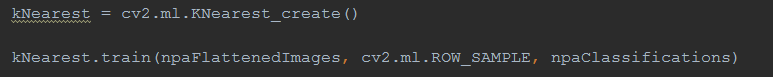
\includegraphics[width=0.6\textwidth]{Pictures/8.png}
\caption{آموزش}
\label{ml}
\end{figure}

\subsection{تشخیص متن}
بعد از خواندن عکس مورد نظر برای تست کردن و اعمال کردن فیلتر های سیاه سفید، گوسی و سپس عبور دادن رنگ های سفید ، کانتور های موجود در عکس را استخراج می نماییم و به آن ها مشخصات 
\lr{(x,y,width,height) }
را برای استفاده بهینه تر نسبت می دهیم. سپس با استفاده از یک حلقه روند تشخیص را شروع می نماییم

\textbf{نکته: }
ابتدا برای پردازش روی عکس های نوشته شده با دست، یک مستطیل دور کانتور های درون عکس می کشیم که نمایش دهنده آیتم های آن می باشد و در یک پنجره آن را نمایش می دهیم، که در عکس زیر آورده شده است، اما در نهایت رابط کاربری از  کد حذف شده اند.

حال به ترتیب با کوچک کردن عکس، تبدیل آن به ماتریس یک بعدی  مقادیر صحیح (برای استفاده در الگوریتم تشخیص) و سپس تبدیل حالت قبل به مقادیر 
\lr{float}
آن را به ورودی الگوریتم 
\lr{KNN}
می دهیم که خروجی اسکی کاراکتر را به ما می دهد که به سان شکل
\ref{string}
 آن رابه یک رشته تبدیل میکنیم که بعد از خروج از حلقه کانتور ها تمامی مقادیر رشته ای را به هم چسبانده و آن را بر میگرداند.مثالی از این برنامه در شکل 
\ref{final}
آمده است.
\begin{figure}
\centering
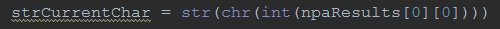
\includegraphics[width=0.6\textwidth]{Pictures/9.png}
\caption{کاراکتر خروجی}
\label{string}
\end{figure}

\begin{figure}
\centering
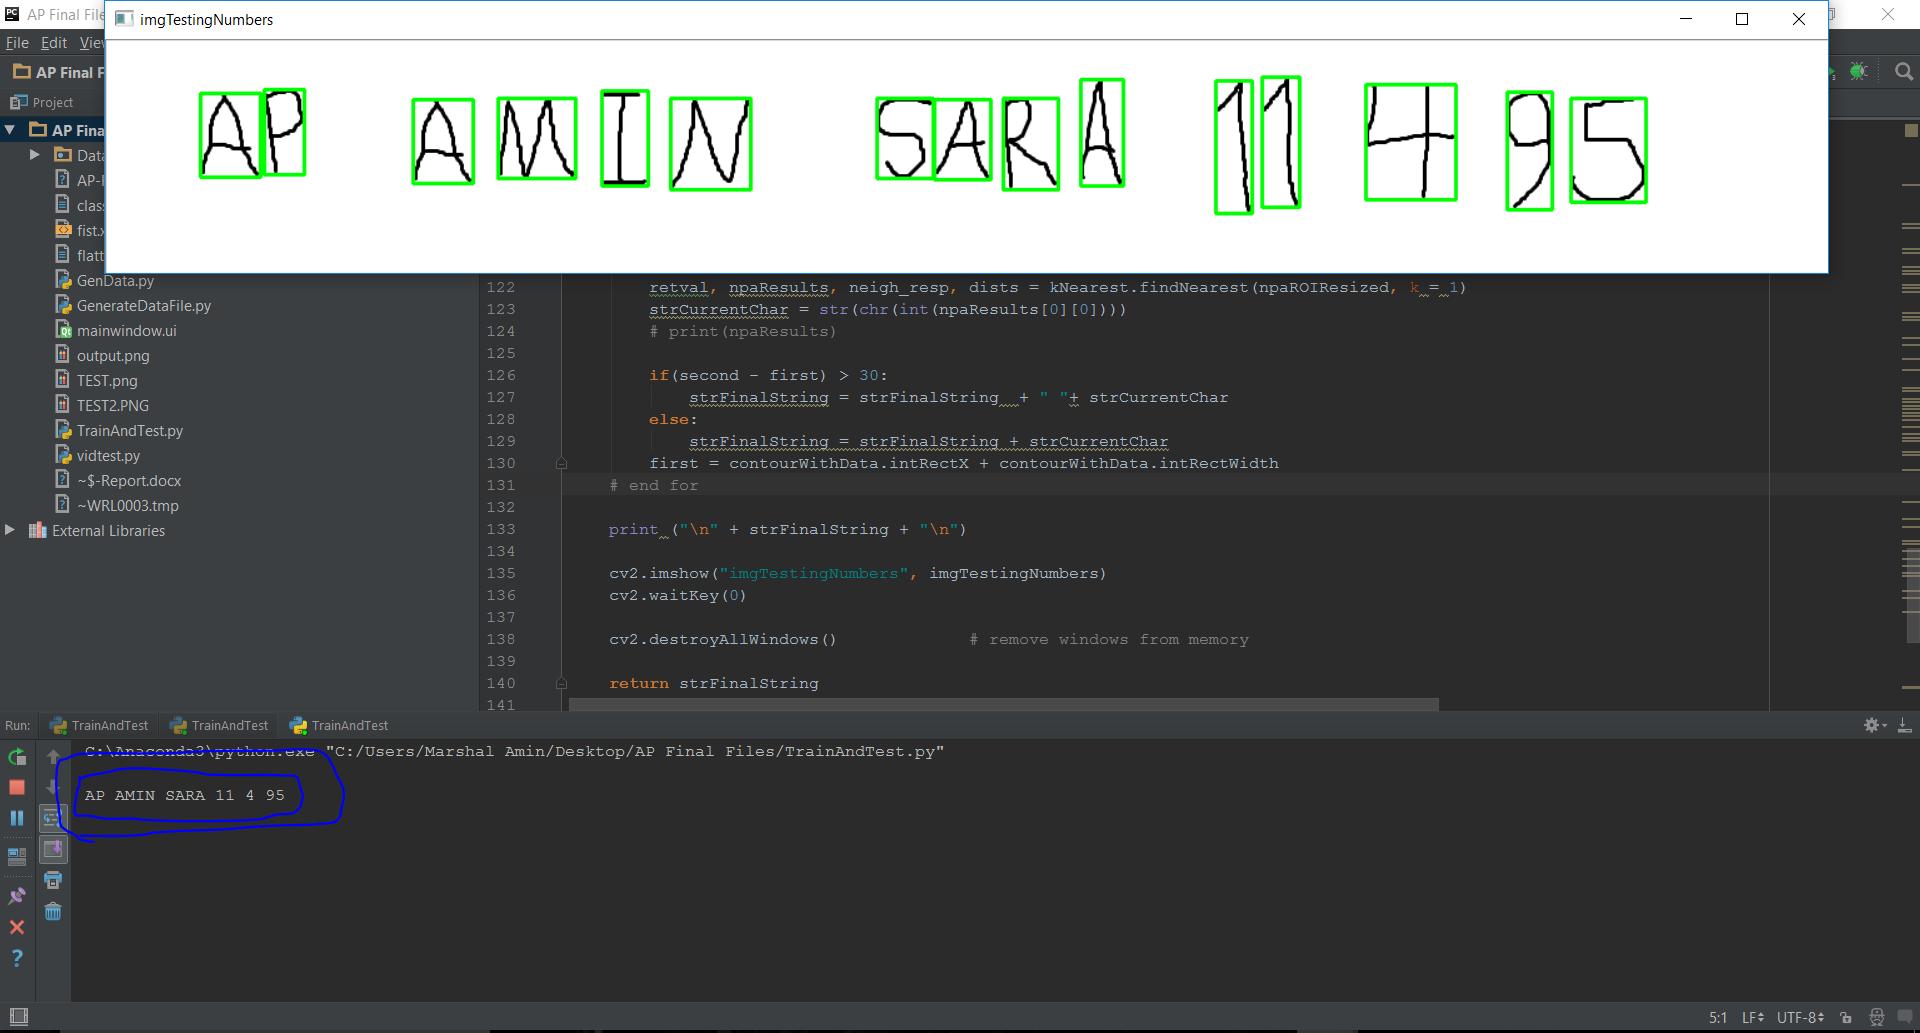
\includegraphics[width=0.6\textwidth]{Pictures/10.png}
\caption{رشته خروجی نهایی}
\label{final}
\end{figure}

\end{document}